\documentclass[conference]{IEEEtran}
\usepackage{cite}
\usepackage{amsmath,amssymb,amsfonts}
\usepackage{booktabs, multirow}
\usepackage{algorithmic}
\usepackage{graphicx}
\usepackage{textcomp}
\usepackage{xcolor}
\usepackage{comment}
\usepackage{wrapfig}
\usepackage{capt-of}
\usepackage[hyphens]{url}
%A set of custom commands that are used for my personal latex style
%Created: Feb 2020
%Updated: July 2020
\usepackage{listings}

\newcommand{\defn}[1]{\textbf{#1}} %definitions are bold
\newcommand{\jnote}[1]{\textcolor{blue}{Justin: #1\\}} %a note from Justin
\newcommand{\rnote}[1]{\textcolor{orange}{Ron: #1\\}} %a note from Ron
\newcommand{\pnote}[1]{\textcolor{purple}{Peyton: #1\\}} %a note from Peyton
\newcommand{\todo}[1]{\textcolor{red}{TODO: #1\\}} %a todo note

\definecolor{tangerine}{RGB}{245,166,35} %comments, primary color
\definecolor{blueSeaFoam}{RGB}{80,227,194}
\definecolor{liteGreen}{RGB}{184,233,134 }
\definecolor{royalBlue}{RGB}{74,144,226} %keywords
\definecolor{amaranth}{rgb}{0.9, 0.17, 0.31} %special keywords
\definecolor{lavender}{rgb}{0.71, 0.49, 0.86}

\lstdefinestyle{mystyle}{
    backgroundcolor=\color{white},   
    commentstyle=\color{black},
    keywordstyle=\color{royalBlue},
    identifierstyle=\color{black},
    numberstyle=\tiny\color{gray},
    basicstyle=\ttfamily\footnotesize,
    breakatwhitespace=false,         
    breaklines=true,                 
    captionpos=b,                    
    keepspaces=true,                 
    numbers=left,                    
    numbersep=5pt,                  
    showspaces=false,                
    showstringspaces=false,
    showtabs=false,                  
    tabsize=2,
    frame=lines,
    %just for Chisel
    emph={Module, IO, Input, Output, UInt, Bool, Wire, Vec, before, after, extend, in, register, insert, apply, Pointcutter, AfterToken, AfterState, Some, when, :=, &&},
    emphstyle=\color{amaranth}
}

\lstset{style=mystyle}

\def\BibTeX{{\rm B\kern-.05em{\sc i\kern-.025em b}\kern-.08em
    T\kern-.1667em\lower.7ex\hbox{E}\kern-.125emX}}

% Ensure letter paper
\pdfpagewidth=8.5in
\pdfpageheight=11in

%%%%%%%%%%%---SETME-----%%%%%%%%%%%%%
\newcommand{\iscasubmissionnumber}{1313}
%%%%%%%%%%%%%%%%%%%%%%%%%%%%%%%%%%%%

\pagenumbering{arabic}

%%%%%%%%%%%---SETME-----%%%%%%%%%%%%%
\title{Feature-Oriented Caches through Feature-Oriented Finite State Machines}
\author{\normalsize{ISCA 2023 Submission
    \textbf{\#\iscasubmissionnumber} -- Confidential Draft -- Do NOT Distribute!!}}
%%%%%%%%%%%%%%%%%%%%%%%%%%%%%%%%%%%%

\begin{document}
\maketitle
\thispagestyle{plain}
\pagestyle{plain}



%%%%%% -- PAPER CONTENT STARTS-- %%%%%%%%
\def\Riscv{\mbox{RISC-V}}
\def\Riscvmini{\mbox{\Riscv{} mini}}
\def\Rocketchip{\mbox{Rocket Chip}}

\long\def\Omit#1{\relax}
\begin{abstract}
\Omit{We investigate the generation of featureful and reconfigurable hardware cache designs. The hardware cache is ubiquitous in computing, yet the designs can vary wildly in different applications, from embedded systems to server grade processors. Instead of each design being unique, why not evolve the design with the features for application? However, as the features get more complex, such as write-through onto a read-only cache or write-back onto a write-through cache, so too must the control structures. 

To this end, we developed a technique to feature-orient finite-state machines. Inspired by aspect-oriented programming, we apply incremental changes to the states and edges of a finite-state machine to alter and customize its behavior in response to features of interest. Thus, allowing efficient specification and generation of numerous designs, each containing only those features of interest for a particular application. We show that our approach can generate designs that are exponentially large in the size of their specifications. In addition to that significant design leverage, the resulting finite-state machines enjoy all the closure properties and proof opportunities for regular languages.

Following from this, we explore the generation of feature-oriented cache designs by combining our feature-oriented finite-state machine technique and prior work in feature-oriented hardware generation. Through this combination, we take an additive approach to our cache design. Rather than rewriting large portions of the hardware generator, we reuse other features to construct new ones. In our results we show 10 separate design endpoints for a small RISC-V processor across both the instruction and data caches.}
We propose a novel methodology for designing and implementing caches.  In lieu of a monolithic specification that contains all features of interest for a given implementation, this approach borrows from aspect-oriented programming, allowing features to be specified such that they can be composed to arrive at a desired implementation.

To achieve this goal, we leverage programming language types and finite-state machine states as hooks for feature specification and deployment.  This allows various implementations of a given cache feature, such as eviction strategy, to be woven easily into a cache design for synthesis and experimentation.   any cache line eviction strategy can be woven into the cache design
Our approach accommodates immediate integration of cache components and their variations, as each feature is woven automatically into a base implementation.

This approach can open a new and competitive marketplace for feature implementations, some formulated for specific application environments, while all can share a common base specification.  Moreover, research ideas can be quickly deployed and evaluated by writing new features that integrate with existing ones.  Those ideas are in turn easily woven into a commercial cache written using our approach. 

We designed and implemented such a cache for the \Riscv{} architecture, available in the \Riscvmini{} implementation.  We thus leverage the
Chisel and Scala platforms to weave features at hardware-generation time using a library we present here, rather than having to develop a new aspect-oriented hardware design language.

We present results from this implementation when synthesized \rnote{blah blah blah}.

\end{abstract}


\section{Introduction}

In their 2018 Turing award lecture, John Hennessey and David Patterson advocated for the adoption of the \Riscv{} architecture by industry and research~\cite{HPTuring}, for applications ranging from embedded processors to supercomputers.  Arguments in favor of such adoption include the following:
\begin{itemize}
    \item Researchers' results (\textit{e.g.}, instruction counts,  cycles per instruction) published using \Riscv{} can be more meaningfully compared because they are based on a common instruction set.
    \item The design of the \Riscv{} ISA allows for elision of features not needed to obtain small footprint for embedded systems.
    \item Ideas developed in research can more easily be adopted by industry when both use a common architecture.
    \item \Riscv{} is simple, easily taught and learned.  A simple processor could be designed and implemented in a single semester.
    \item Common toolchains (such as the \texttt{gcc} suite~\cite{gcc}) already target \Riscv{}.
    \item Reference implementations exist for \Riscv{}~\cite{chisel:riscv,RvMini} that have been rigorously tested.
    \item Special-purpose hardware accelerators have been designed using \Riscv's coprocessor interface~\cite{accels}.
\end{itemize}
While these goals are certainly attractive, it is nonetheless a daunting task to modify a characterization of \Riscv{} to add or subtract features.  A large number of implementations of \Riscv{} currently exist~\cite{riscvimplementations}.  Each is generally a separate characterization intended to support applications of interest.  The following implementations are of the greatest relevance to our work:
\begin{itemize}
   \item \Riscvmini{}~\cite{RvMini} is a 3-stage pipelined implementation of 32-bit \Riscv{} processor. It lacks many features that might be desirable for performance, but it is a relatively simple and easily understood implementation.  It includes instruction and data caches, but it omits floating-point support.  It is well documented and highly suitable for use in courses.
   \item \Rocketchip{}~\cite{chisel:riscv} is a robust implementation of 64-bit \Riscv{} using a 5-stage pipeline.  Its microarchitecture offers many features that improve performance and support larger applications, such as an MMU and floating-point arithmetic.  The intended applications include systems-on-a-chip (SoC).
   \item Boom~\cite{boom} is an adding out-of-order execution implementation of \Riscv{}. Although it shares some of the same libraries as \Rocketchip{}, it is a separate implementation with much functionality that duplicates the core functionality of \Rocketchip{}.
\end{itemize}
From the first to the last, these implementations add features to create an increasingly sophisticated implementation of \Riscv{}.  Each is written using the hardware generator language Chisel~\cite{chisel:book}, which is in turn embedded in the programming language Scala~\cite{scala-overview-tech-report}.  The execution of a Chisel program generates a hardware description, and the desirable features of modern, high-level languages are available in Chisel.  Both of these advantages are relevant to our work.

The features available for a given \Riscv{} processor are present in the code base and characterization for that processor.   There are configuration tools such as Diplomacy~\cite{diplomacy} that help parameterize the \Rocketchip{} processor and appropriately connect components to form an SoC. 

In our approach, features are defined so that they can be \emph{woven} into an implementation (a base characterization along with features already chosen and deployed) using well-defined type and state information.  For example, \Riscvmini{} already provides an instruction and data cache.  While most implementations would find those caches useful, we note the following:
\begin{itemize}
    \item It may be useful for pedagogical purposes to define the processor without the complexity of a cache already in place.  We can instead load and store from a simple (and necessarily small) memory to simplify the overall processor specification.  The cache can be subsequently introduced.
    \item The inclusion of a predefined cache makes it difficult to modify \Riscvmini{} to use a \emph{different} cache.  For experimentation that holds all else constant but seeks to evaluate different cache implementations, it is burdensome an error-prone to modify \Riscvmini{} to incorporate a different cache. 
\end{itemize}
In a feature-oriented approach, the evolution of a base implementation to include a cache eventually might proceed as follows:
\begin{itemize}
    \item The base implementation includes an abstract definition (a \emph{trait} in Chisel/Scala) that represents fetching values based on an address.  That trait is then extended to allow for storing data at a given address.  
    \item Any implementation that implements those traits is (type) suitable to serve as the mechanism for implementing loads and stores.
    \item Initially, a small scratchpad memory could be deployed, which accommodates exposition and testing of the rest of the processor.
    \item Subsequently, any cache that implements the traits can serve to handle loads and stores.  One such implementation can be the one currently provided with \Riscvmini{}.
    \item Experimentation can proceed with any number of cache implementations, each incorporated into an instance of a \Riscvmini{} processor.
\end{itemize}
This approach does not come for free and it requires the following development methodologies:
\begin{itemize}
    \item A base implementation and its features must contain sufficient types and states so that other features can use those as hooks for deployment.
    \item Newly conceived features may require refactoring both the base implementation and affected features, to provide necessary hooks for a new feature's deployment.
\end{itemize}
Continual refactoring is seen as an advantage in the software world, as it raises the abstraction level of a project and tends to clarify logic and purpose of code. We provide examples of such refactoring in this paper. \rnote{the interception of loading a line to make a copy for dusty caches}

In this paper we use the above ideas to develop a feature-oriented cache and we present results from its deployment in \Riscvmini{}.  \rnote{Caches provide lots of parameters and choices to play with.  if we're successful we get a marketplace.  easier to describe, implement, and teach.}

\rnote{contributions}

\rnote{roadmap...
Todo: aop, why chisel, the library useful for other things}

\section{Prior Work}

\subsection{Chisel, Scala, FIRRTL}

Most hardware designs, including caches, are specified using hardware \emph{characterization} languages such as Verilog~\cite{verilog} and VHDL~\cite{vhdl}.  While those languages offer some abstractions in the form of parameters and restrictive loops, they lack abstractions such as classes, traits, and types that allow cleaner and more robust specifications of software systems.  To a cache using a hardware characterization language, we would have to build a tool that allowed high-level specification of cache features, from which we could then generate a design of interest.

Hardware generation languages like Chisel, on the other hand, allow the designer to write a program whose execution generates a design.  Chisel, based on Scala, has abstractions such as types, classes, and traits that allow a richer specification of a cache.  For example, the interface from cache to memory can be captured by a trait that captures the address and data to be transferred.  Any implementation of that trait suffices to be the ``memory'' backing a cache.

Transformations of the hardware design, for example to weave in features of interest, can be accomplished at the Scala level (using Scala meta) or FIRRTL level (using tree operations on Chisel's intermediate form).

\subsection{Aspect-Oriented Programming}

Large software systems are subject to the ``tyranny of the dominant decomposition'' in that the objects and methods that form the nouns and verbs of the system are those that are most present in the design.  Such systems, however, often have cross-cutting concerns.  For example, a log of class and method activity can require action at each method's call and return.  Aspect-oriented programming (AOP)~\cite{Kicz97} allows the specification of \emph{join-points} to model method calls and returns, along with \emph{advice} that specifies what should be done at those points of execution.  A general specification of a set of join-points is called a \emph{pointcut}. AspectJ~\cite{AspectJ:01} is a robust implementation of an AOP using Java.

For our work, AOP provides the approach we need to modifying finite-state machines, such as the one controlling a cache, to incorporate features as desired.  
Internally, the cache's operation is governed by a finite-state machine.  Features are woven into the design as modifications of the finite-state machine (a base specification along with other features of interest).

Aspects and FSMS have been used to describe the evolution of software product lines, with the goal of determining whether aspect application would terminate, and, if so, whether the results are sensitive to the order of application~\cite{aspectsUML}.

Closer to our work, aspects and FSMs have been previously combined to reason about the interactions of a system's features~\cite{6078174}.  We take a common approach to specifying how FSMs are modified, which we explain below, based on states, transitions, and labels (symbols) of an FSM.  Their work is concerned with showing incompatibility of features (for example, call-waiting, and three-way calling).  In other words, they model the actions of larger system using an FSM.  Our cache controller \emph{is} the FSM of interest, and we use aspects to build up its functionality.   Incompatible features in our world are resolved by the first to modify the FSM, because thereafter the hook is no longer available.

\subsection{FOP in software systems}
Our approach to cache design is influenced by the success of this idea in the software world.  For example, a CORBA event channel~\cite{corbaeventchannel} offers many features in a complete implementation, but a given application may need only a few of those features.  Using an aspect-oriented approach, features were incorporated as desired, yielding implementations whose footprint and delay are affected only by necessary features~\cite{ourwork}.  That work shows that by omitting unnecessary features, implementations can be generated that take much less area (code) and that have significantly better performance (latency) than the full-featured, monolithic version.  That work used the aspect compiler AspectJ~\cite{AspectJ:01} and a code base for an event channel and its features written in Java~\cite{Java}.
\rnote{results from the above here?}


\section{Feature-Oriented Finite State Machines} \label{Sec:FSM}

FSMs serve as the basis of control for many components of an architecture implementation, including cache control and multi-cache coherence, bus arbitration, and network protocols.  We review the formalism of  FSMs and then describe how aspects can transform such machines to implement features of interest.  We then describe a library we have implemented in Scala/Chisel to simplify expression of aspects for FSMs.  When run as a Chisel program, the resulting FSMs synthesize Verilog with the features of interest.

\subsection{High-level Overview}
An FSM $M$ is typically defined as follows: 
\[M = (Q, \Sigma, \delta, q_0, F)\]where $Q$ is a set of states, $\Sigma$ is a set of tokens, $\delta$ is the transition function, $q_0$ is the start state, and $F$ is the set of accepting states.  A state is typically denoted by an upper-case letter;  lower-case letters denote tokens and strings. \rnote{our diagrams do not follow this notation; I propose we drop the previous two sentences.} The symbol $\lambda$ denotes the empty string.  When an FSM is drawn as a graph, states are shown as nodes and transitions as labeled edges.  The start state receives an edge with no source, and an accepting state is drawn with two concentric circles. 

\subsubsection{Decidability and Testing}
For regular languages and (thus) FSMs, questions of interest about machine behavior are decidable~\cite{sipser}.    For example, consider a feature that is intended to \emph{extend} the behavior of a design, so that all previous inputs are allowed, but the feature introduces some other allowable inputs.
An example here is an FSM that scans characters to parse them as decimal numerals.  A feature might extend that syntax to accommodate hexadecimal numerals for inputs that begin with \texttt{0x}.  With our approach, the introduced feature creates a new FSM, whose language is provably a proper superset of the original FSM's language.  As another example, \emph{timed automata}~\cite{10.1145/2518102} could reason about real-time properties of finite-state machines generated by our approach.  The ability to reason about modified FSMs and their behavior can greatly reduce the need for testing.  We do not rely on this advantage in our work, but this is one reason FSMs are attractive for hardware designs.


\subsection{Finite-State Machine Aspects}

We follow~\cite{aspectsUML} in the treatment of aspects for FSMs. Essentially, a state is like a method and a transition between states is like a method call.  We next describe the specific formulation of aspects for FSMs.  

As an example to show the advantages of an AOP approach for cache designs, consider the imposition of a write-back feature for a cache.  The feature requires modification of the cache design in multiple places:
\begin{itemize}
    \item A line of cache must contain a dirty bit.
    \item The dirty bit must be set if the program modifies any byte in the line.
    \item When a line is replaced, the dirty bit must be consulted to determine if the line must be written back to the backing storage.
\end{itemize}
With an AOP approach, these changes are expressed together in a write-back feature, whose inclusion affects the FSM appropriately as described above.  The elements of the feature are:
\begin{itemize}
    \item A \emph{pointcut} specifies where in the FSM changes should occur.  The pointcut then yields a set of$\ldots$
    \item Join points, which are specific states or transitions in the FSM, at which$\ldots$
    \item Advice in the form of FSM modifications are applied.
\end{itemize}

\subsubsection{Pointcuts}
Pointcuts are either a set of states or a set of transitions in the FSM that satisfy some predicate. Predicate $p$ can determine the members of the pointcut by any user accessible attributes of a Scala object. For example, $p$ may be a type, trait, or even a value of an instance variable. It is likely that the base code requires refactoring to include this type information. However, the effort is worthwhile because the refactoring allows for richer and more precise pointcuts.

State pointcuts are analogous to a set of function bodies in a program. Just as a function body is unique within a program, each state join-point within the pointcut will also be unique. Token pointcuts are analogous to a set of function calls. Unlike function bodies, function calls may appear many times within a program. This is also true for a token within a FSM. Thus, the resulting pointcut will contain all the \emph{transitions} where the predicate $p$ was satisfied. 

\subsubsection{Advice}
Building on the analogy in the previous section, one can think of a FSM as a series of function bodies (states) where function calls (transitions) come at the end of the body (i.e. continuation-passing style). Advice gets inserted into the execution flow in this analogy. After the application of advice, the program would be required to pass through the advice or be directed somewhere else. In terms of the FSM this means that control is changed or paths to different states are changed.

We consider the usual forms of around, before, and after advice (\emph{cf}. AspectJ~\cite{AspectJ:01}). Around advice takes the joinpoint and replaces it with something else. States replace states and transitions replace transitions. Before and after advice come in the form of token-state or state-token pairs in order to add a new path through the FSM. Figure \ref{fig:adviceExamples} shows the effect of different types of advice on a toy FSM. Before advice (q3, e) on q1 takes all paths into q1 and directs them into q3, on e the machine transitions to q1. The reverse is true for after advice (e, q3) on q1. All paths leaving q1 now leave q3 and the transition from q1 to q3 takes place on e. Similarly, before advice (e, q3) on a places e going into q3 and a out of q3. The reverse is true for after advice (q3, e) on a.

\begin{figure}[ht]
    \centering
    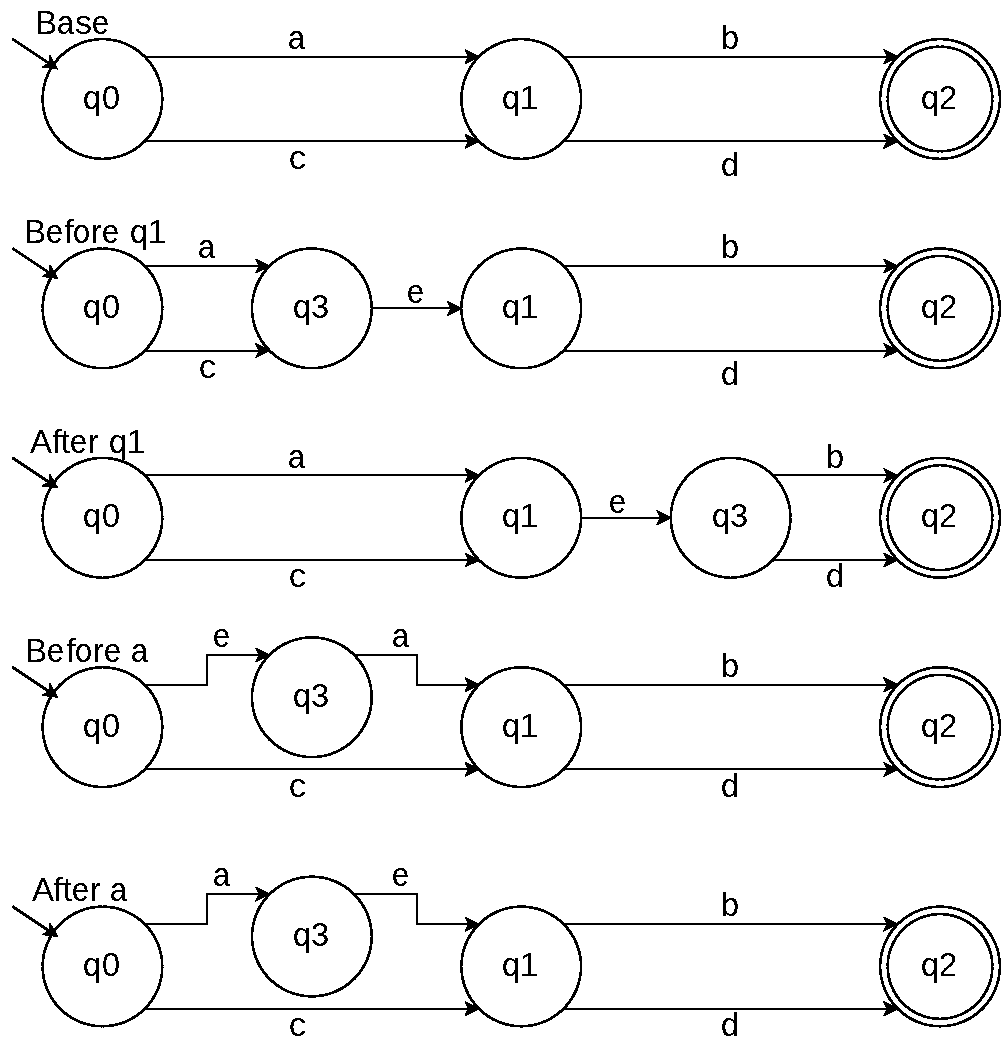
\includegraphics[width=0.5\textwidth]{isca2023-latex-template/figures/AdviceExamples.drawio.pdf}
    \caption{Examples of before and after advice on a small toy FSM.}
    \label{fig:adviceExamples}
\end{figure}

\subsubsection{Context aware advice} 
Our advice can also be conditioned by the immediate context around it. State advice is aware of the paths going into and out of the state it is affecting and token advice is aware of the states preceding and seceding the transitions each token is involved in. For example the before advice on state q1 in Figure \ref{fig:adviceExamples} could have two different paths placed before q1 depending if it was affecting a or c. This allows for very dynamic advice creation for changing the control structures for hardware.

\subsection{Software Library}\label{sec:foam}
All the mechanics described in Section \ref{Sec:FSM} have been built into a software library. Since we targeted Chisel for hardware generation, this library is also built in Scala. As is, it can be dropped into any Chisel hardware generator to construct and generate hardware FSMs. The software library contains a set of base classes, \texttt{FSM}, \texttt{state}, and \texttt{token} that can be arbitrarily extended by end users to fit their construction needs. 

Furthermore, the library fully handle all feature application through our \texttt{Weaver} class (in AOP, code is ``woven'' into a codebase). Just like aspect compilers, our weaver continues to apply advice until the resulting FSM is the same as the previous iteration. Advice may introduce new joinpoints within the FSM making it necessary to reapply the aspects that contain those join-points in their pointcuts. Thus, just like aspect compilers, it is possible to create an aspect that infinitely applies to the FSM, which end users must be careful of.

\subsubsection{Writing Aspects for Finite-State Machines}
We have modeled the programming interface off the well established aspect language for Java, AspectJ~\cite{AspectJ:01}. This gives a familiar interface for aspect practitioners, as well as connects with prior AOP languages. We did not have to create any new syntax to implement our library; everything is in plain Scala/Chisel.

\paragraph{Pointcuts}
Figure \ref{fig:pointcut} demonstrates the creation of a hypothetical pointcut. Here, the predicate is written using a plain Scala \texttt{match} statement. The \texttt{Pointcutter} will iterate over all the states in the FSM and add them to the pointcut if the predicate evaluates to true. A predicate can be written as any arbitrary Scala code as long as it follows the interface of consuming a state (or token) and returns true if it satisfies the properties defined in the predicate. The result of this example would create a pointcut containing a set of \texttt{ReadState} objects where the threshold was higher than some value stored in the object.

\begin{figure*}[ht]
    \centering
    \begin{lstlisting}[language = Scala]
val statePointcut = Pointcutter[State, ReadState](fsm.states, state => state match {
  case s: ReadState if(s.value <= threshold) => true
  case _ => false
})
    \end{lstlisting}
    \caption{A hypothetical pointcut in our software library.}
    \label{fig:pointcut}
\end{figure*}

\paragraph{Advice}
Figure \ref{fig:advice} shows the construction of advice using the \texttt{AfterState} class. Any arbitrary Scala code can be executed inside the advice body as long as it returns advice. \texttt{StateJoinpoint} provides reflexive access to the join-point as well as its context. This advice, in conjunction with the \texttt{statePointcut} from Figure \ref{fig:pointcut}, would create a transition from every state in the pointcut to \texttt{FlushState} on \texttt{ready}. 

\begin{figure*}[h]
    \centering
    \begin{lstlisting}[language = Scala]
AfterState[ReadState](statePointcut, fsm)((thisJoinPoint: StateJoinpoint[ReadState], thisFSM: FSM) => {
  
    (Some((ready, FlushState)), thisNFA)
})
    \end{lstlisting}
    \caption{A hypothetical advice in our software library.}
    \label{fig:advice}
\end{figure*}

\subsubsection{Hardware Generation}
Our software library uses Chisel constructs to generate hardware FSMs. These are the exact same hardware constructs that Chisel uses under the hood to generate their hard coded FSMs. Before generation, end users associate each state and token with a string ID. Then, each state is given a conditional block and the transitions placed inside with their own conditional blocks. The end user is returned a handle to the FSM. The handle has one wire associated with each state. This signal is asserted when the state becomes active. The handle also has one assignable wire for each token. When this signal is asserted and it is associated with current active state, the transition occurs.

In Figure \ref{fig:handle} we show how an FSM handle might be associated with both a state and a token. Since the FSM interacts with the outside world via a handle, the \emph{implementation} of what happens when a state is asserted is completely decoupled from the FSM itself. This is extremely useful from a feature-orientation standpoint. New implementation information can be added as features are added. As long as the FSM's handle remains in scope and a \texttt{module} barrier is not crossed, the signals in the handle can be used anywhere. 

\begin{figure*}[ht]
    \centering
    \begin{lstlisting}[language = Scala]
when(fsmHandle("sReadCache")) {
  when(hit) {
    io.resp.valid := true.B
  }
}

fsmHandle("readFinish") := !io.req.valid && hit
    \end{lstlisting}
    \caption{Using an FSM handle in our software library.}
    \label{fig:handle}
\end{figure*}

\begin{comment}
\subsection{Case Study: Vending Machine}
As an example of a featureful FSM we present the case study of the control of a vending machine. A state in our design carries the necessary (Scala) \emph{traits} to represent its role in the machine's operation:  the funds inserted and the potential products dispensed.
For this example and the results we present, the features of interest for a vending machine are as follows:
\begin{itemize}
    \item \textbf{Add Currency} introduces a value of coinage.
    \item \textbf{Dispense Product} introduces a vendible item and its price.
    \item \textbf{Print Funds} causes the machine to display the total funds after each state change.
    \item \textbf{Insufficient Funds} introduces a prompt to advise the consumer to insert more funds to buy a particular item.
    \item \textbf{Change Return} introduces a button (input to the FSM) that causes the machine to return unspent funds.
    \item \textbf{Peanut Warning} requests confirmation of purchase for items that contain peanuts.
    \item \textbf{Buy More} allows the consumer to continue purchasing items if funds remain in the machine.  The \textbf{Change Return} feature, if present, allows the consumer to request return of the remaining funds.
\end{itemize}

A monolithic approach requires designers to specify all states and transitions for each feature subset, which is tedious and error-prone. With our approach, designers can verify the correctness of much smaller designs and then obtain much larger generative designs that are correct by their construction.

In terms of leverage, consider an FSM for which there are $n$ orthogonal and independent features.  A valid system could thus be written or generated with or without each of those $n$ features.  This leads to $2^{n}$ feature-specific implementations.  While it is unlikely that each of those implementations would find an application, the ability to generate \emph{any} of them automatically offers significant leverage.

We implemented all the features in our library. The resulting FSMs were then emitted as Verilog. The Verilog was synthesized on a xc7a35tcpg236-1 FPGA using Vivado 2022.1. Below we report the number of generated states, transitions in the FSM, and the space in LUTs that the FSM took up in on the FPGA.

Figure~\ref{fig:vmData} shows the results for different endpoints generated by our library. For our tests, we held the currency threshold at 100. Every machine contains 5, 10, and 25 value coins; and 4 products of value 25, 50, 75, and 100. This is captured by \emph{None}. In the first set of results, each feature is shown by itself. Even single features can greatly increase the components in the FSM. The \textbf{Buy More} feature (denoted B) by itself more than doubles the number of states and transitions. This impressive leverage is further exemplified when combining features. 

In these cases the number of states increase by 2.5x in the simplest endpoint up to 4.6x in the most complex, and the transitions by 2.5x and 5x respectively. Recall, this is in a relatively simple vending machine that can only accept up to 100 units of value. Simply doubling the amount of accepted value to 200 creates a machine with 284 states (10.5x increase over the base) and 3113 transitions (16x increase over the base). However, this is accomplished in our library with relatively few lines of code. The largest feature in terms of code is \textbf{Peanut Warning}, which is implemented in just 39 lines.

Despite the growing number of generated states and transitions as the features increase in Figure~\ref{fig:vmData}, the resulting hardware resources, in this case Look Up Tables (LUTs), used by the FSM are relatively modest. This is because hardware synthesis tools can represent states using a linear encoding scheme.  For an FSM with $n$ states, each state takes only $O(\log{n})$ space when encoded as an integer.  However, the \emph{specification} of that circuit to a synthesis tool must be expressed state-by-state.  If the number of transitions per state is bounded by a constant, then the specification (\textit{e.g.}, lines of Verilog) takes $O(n)$ space.  Our generative approach to hardware FSMs opens hardware designers to implementing much larger FSMs than are currently sustainable with a hand-coded approach.

\begin{figure}
    \centering
    \scriptsize
\begin{tabular}{lrrrr}\toprule
Features &States &Transitions &LUTs \\\midrule
None &27 &208 &24 \\
P &47 &368 &38 \\
I &47 &368 &46 \\
C &48 &423 &70 \\
W &33 &320 &60 \\
B &57 &448 &60 \\
PI &67 &528 &73 \\
PICB &118 &1053 &186 \\
PICW &94 &1023 &160 \\
PICWB &124 &1353 &220 \\
\bottomrule
\end{tabular}
    \caption{Number of generated states, transitions, and LUTs depending on selected features. The features are as follows: P = Print Funds, I = Insufficient Funds, C = Change Return, W = Peanut Warning, and B = Buy More.}
    \label{fig:vmData}
\end{figure}
\end{comment}

\section{Feature-Oriented Cache}
\begin{figure*}[ht]
    \centering
\scriptsize
\begin{tabular}{llll}\toprule
&Endpoint &Features \\\midrule
\multirow{2}{*}{Instruction Cache} &Read-Channel &HasWriteStub, HasBufferBookeeping \\
&Read-Only &HasWriteStub, HasMiddleAllocate \\\midrule
\multirow{5}{*}{Data Cache} &Write-Channel &HasWriteFSM, HasSimpleWrite, HasBufferBookeeping, HasInvalidOnWrite \\
&WriteBypass &HasWriteFSM, HasSimpleWrite, HasMiddleAllocate, HasInvalidOnWrite \\
&WriteThrough &HasWriteFSM, HasSimpleWrite, HasMiddleAllocate, HasMiddleUpdate \\
&WriteBack &HasWriteFSM, HasSimpleWrite, HasMiddleAllocate, HasMiddleUpdate, Dirty Accounting \\
&Dusty &HasWriteFSM, HasSimpleWrite, HasMiddleAllocate, HasMiddleUpdate, Dirty Accounting, Dusty \\
\bottomrule
\end{tabular}
    \caption{Endpoints for the Instruction and Data Caches.}
    \label{fig:Endpoints}
\end{figure*}

Overcoming the hurtle of evolving the control structures allows us to then feature-orient the cache as a whole. The feature-oriented cache presented here prototypes our hardware generation technique that we believe increases modularity, design reuse, and shareability.

\subsection{Feature Decomposition}
The stateful nature of the cache requires feature decomposition across both the internal hardware and the FSM that controls it. However, the instruction and data cache designs are not mutually exclusive. They both share the same base design for both the FSM and the cache overall. All endpoints for either cache are the result of applying features to the same base designs. All our designs are built for the RISC-V Mini processor~\cite{RvMini}. The RISC-V Mini is a single issue 3 stage pipelined processor. 

We strategically chose this processor, despite its small size. A goal of feature-oriented programming is to begin with a small design and then \emph{additively} build upon it. So, we chose RISC-V Mini rather than a complicated chip generator like Rocket Chip~\cite{chisel:riscv} to save us the time of tearing down the fully-featured implementations already present in these generators.

\subsubsection{Finite-State Machine}
We have divided the FSM's mechanisms into five seperate features.
\begin{itemize}
    \item \textbf{Read} provides all the functionality for a read-only cache. 
    \item \textbf{Write} provides the functionality to write to memory. This is an \emph{abstract feature}. By itself it does not have enough to complete cache transactions. One of the two following features must also be included.
    \item \textbf{Acknowledge Idle} returns the cache back to the idle state after the backing store acknowledges a write.
    \item \textbf{Acknowledge Read} returns the cache back to the read state after the backing store acknowledges a write.
    \item \textbf{Dirty Accounting} provides the necessary transitions for a write-back cache.
\end{itemize}

Since the generator itself calls into our software library, all of our FSM features are subsumed into our hardware generator features (discussed in Section \ref{sec:hwFeatures}). 

\subsubsection{Hardware Generator}\label{sec:hwFeatures}
Below are the 9 separate hardware generation features for our cache. In all cases, the cache implements the AXI~\cite{AXI} interface for communication with the backing store and follows the request-response interface already present in the RISC-V Mini datapath.

Note, to show the extensibility of our feature-oriented approach we have also included the \textbf{Dusty}~\cite{Krishna:06, Friedman:05} feature. Instead of writing any dirty line back to memory, a dusty cache will a secondary ``image'' of main memory to see if the line has actually changed since it was first brought into cache. This is useful with circular counters as they frequently return to the same value.

\begin{itemize}
    \item \textbf{Base System} provides the structure to which all other features can be applied.
    \item \textbf{HasBufferBookeeping} enables just enough bookkeeping to hold one buffered memory transaction.
    \item \textbf{HasMiddleAllocate} builds out the internal memory for the cache and allows cache lines to be allocated.
    \item \textbf{HasWriteStub} stubs off the write channel for read-only memory.
    \item \textbf{HasWriteFSM} introduces the write FSM with both the \textbf{write} and \textbf{Acknowledge Idle} features applied.
    \item \textbf{HasSimpleWrite} provides the hardware necessary to write to memory.
    \item \textbf{HasInvalidOnWrite} invalidates the buffer or cache line if the tag matches.
    \item \textbf{HasMiddleUpdate} allows the internal memory of the cache to be updated by writes from the datapath.
    \item \textbf{Dirty Accounting} modifies the FSM with both the \textbf{Acknowledge Read} and \textbf{Dirty Accounting} features. As well as providing all the hardware necessary for handling dirty cache lines.
    \item \textbf{Dusty} creates a second internal memory for the cache that acts as an image of main memory. A cache line is only considered dirty if the internal memory and image of the line are not equal.
\end{itemize}

\subsubsection{Endpoints}

Our features combine to form endpoints for both an instruction and data cache. Endpoints for both the instruction and data caches can exist in the same system at the same time (how this is achieved is discussed in Section \ref{sec:implementation}). This means that our cache system can realize 10 separate overall endpoints, two choices for instruction cache and five choices for the data cache. Figure \ref{fig:Endpoints} lists all of the endpoints for the instruction and data caches, as well as the features combined to achieve each of them. 

The \textbf{Read-Channel} and \textbf{Write-Channel} endpoints implement the hardware necessary for memory transactions as well as a small buffer for use with the AXI interface. In all other cases our generator creates a direct mapped cache with 256 sets and 16 byte cache lines. Set-associative and fully-associative caches are not precluded by our approach, they are just beyond the scope of the experiments in this paper.

\subsection{Feature Implementation}\label{sec:implementation}
In Chisel hardware generators such as RISC-V Mini~\cite{RvMini}, Rocket Chip~\cite{chisel:riscv}, and BOOM~\cite{} we have generally observed a lack of modularity in the generator code. Commonly, the organization of the generation code reflects what would usually be seen in hardware description languages where functionality is hard-coded and entangled with other features. Despite the fact that Chisel is embedded within the Scala language, hardware designers have yet to embrace the full power of object-oriented programming and functional programming. This results in designs that are difficult to extend and reuse due to their high level of specialization. In this section, we present our feature-oriented hardware generation technique that overcomes these issues.

Our implementation combines Chisel, our library, and another aspect-oriented tool, Faust~\cite{Deters:21} that inserts code into Scala programs via abstract-syntax tree modification. We use Faust to apply all of our features \emph{automatically} to the RISC-V Mini codebase. End users can select any of the 10 design endpoints from the command line. Faust takes care of application and un-application of the featuers.

Figure \ref{fig:LOC} lists how many lines of code each it took to implement each of our features. By taking a feature-oriented approach we were able to achieve a high level code leverage and design reuse between features. On average each feature is only 43 lines of generation code. Our largest feature, \textbf{Dirty Accounting} is just 104 lines of code. This feature, by itself, adds all the necessary hardware to build a write-back cache out of a write-through cache.

\begin{figure}[ht]
    \centering
\scriptsize
\begin{tabular}{lrrrrr}\toprule
Feature &Chisel &Our Library &Faust &Total \\\midrule
Base System &336 &25 &0 &361 \\
HasWriteStub &10 &0 &0 &10 \\
HasWriteNFA &10 &55 &0 &65 \\
HasSimpleWrite &17 &0 &0 &17 \\
HasBufferBookeeping &35 &0 &16 &51 \\
HasMiddleAllocate &68 &0 &8 &76 \\
HasInvalidOnWrite &12 &0 &8 &20 \\
HasMiddleUpdate &21 &0 &8 &29 \\
Dirty Accounting &11 &27 &66 &104 \\
Dusty &0 &0 &14 &14 \\
\bottomrule
\end{tabular}
    \caption{Lines of code used to implement each feature.}
    \label{fig:LOC}
\end{figure}

\begin{figure*}[ht]
    \centering
    \begin{lstlisting}[language = Scala]
class Cache(val c: CacheConfig, val nasti: NastiBundleParameters, val xlen: Int) extends Module {
  //outward facing IO
  val cpu = IO(new CacheIO(xlen, xlen))
  val mainMem = IO(new NastiBundle(nasti))

  // local parameters
  protected val p = new CacheParams(c.nSets, c.blockBytes, xlen, nasti)

  //build the NFA for the cache
  protected lazy val cacheNFA = Weaver[NFA](List(), ReadFSM(), (before: NFA, after: NFA) => before.isEqual(after))
  protected lazy val fsmHandle = ChiselFSMBuilder(cacheNFA)

  //this section is for things needed by the frontend and the backend
  //split the address up into the parts we need
  protected val nextAddress = Wire(chiselTypeOf(cpu.req.bits.addr))
  protected val address = Reg(chiselTypeOf(nextAddress))
  ...

  //create a buffer for reads from main memory, also store the tag
  protected val buffer = Reg(Vec(p.dataBeats, UInt(nasti.dataBits.W)))
  //we will always have at least this
  val valids = RegInit(0.U(p.nSets.W))

  //set up phases used in every cache
  protected val front = new Frontend(fsmHandle, p, cpu)
  protected val back = new Backend(fsmHandle, p, mainMem, address)

  //hit can be several different things depending on the feature set
  protected val hit = Wire(Bool())
  hit := false.B
  ...

  front.read(hit)
  ...
}
\end{lstlisting}
    \caption{The implementation of the Cache class.}
    \label{lst:BaseSystem}
\end{figure*}

\begin{figure*}[ht]
    \centering
    \begin{lstlisting}[language = Scala]
trait HasMiddleAllocate extends Cache {
    val middle = new Middleend(fsmHandle, p, address, tag, index, valids)
    val (oldTag, readData) = middle.read(buffer, nextAddress, offset, Some(hit), Some(cpu))
    middle.allocate(Cat(mainMem.r.bits.data, Cat(buffer.init.reverse)), readDone)
}
    \end{lstlisting}
    \caption{HasMiddleAllocate feature.}
    \label{fig:HasMiddleAllocate}
\end{figure*}

\subsubsection{Hardware generation through types}\label{sec:types}
Rather than tying the structure of the hardware generator code to the hardware hierarchy, we propose separating hardware into types with specific generation tasks. To illustrate this, the base \texttt{Cache} class is listed in Figure \ref{lst:BaseSystem}. Here, the \texttt{Cache} class is responsible for creating and initializing the hardware needed for the optional cache features. 

Furthermore, on lines 25 and 26 we have the \texttt{Frontend} class and \texttt{Backend} class. These two classes are responsible for generating the hardware needed for communication with the datapath and the backing store, respectfully. Separating these concerns and encapsulating them into their own classes, they have become decoupled from the rest of the hardware. In the future, if the design moved away from AIX to a different protocol, \texttt{Backend} could be swapped out for a different class that has the same interface, with appropriate changes to the FSM and IO for the module.

Hardware generation types give us a way to \emph{optionally} generate hardware through method class. On line 33 the \texttt{read()} method is called because every cache design must read from memory. However, some endpoints require the ability to read from memory. So, the \textbf{HasSimpleRead} feature calls the \texttt{write()} method of the \texttt{Frontend} while the \textbf{HasWriteStub} feature calls \texttt{writeStub()}. Instead of having to write one implementation for read-only and one implementation for read-write, we can call one method or another while sharing the rest of the design. In addition, the hardware design may easily be extended by adding new hardware generation methods or overriding old ones.

Critically, hardware as types creates ``hooks'' for us to grab onto to modify the abstract syntax trees with Faust. Within our generator, the instruction cache and data cache are \emph{subtypes} of \texttt{Cache}. We direct Faust to modify the cache of a specific type with the desired features. This enables us to easily create endpoints modifying both caches without having to worry about cross contamination of features between the two.

\subsubsection{Features as Traits}
Traits in Scala function similarly to Java interfaces. Unlike Java, Scala traits support multiple inheritance and Scala code can be called from within a trait. Packaging functionality into traits is not a new idea. RISC-V Mini, Rocket Chip, and BOOM all have traits that implement some functionality. However, our approach differs significantly in that we package \emph{whole features} into traits. Thus, to add a feature to a design, the type can just be extended with the trait containing the feature.

Take the \textbf{HasMiddleAllocate} feature in Figure \ref{fig:HasMiddleAllocate}. By extending the \texttt{InstructionCache} with \textbf{HasMiddleUpdate} instead of \textbf{HasBufferBookeeping} the read-channel is transformed into a read-only cache. By combining this with our type encapsulation technique from Section \ref{sec:types}, zero hand rewriting of the design is required to make this extensive change.

Since Faust modifies the abstract syntax tree of the hardware generator, creating different endpoints only requires instructing Faust to extend the cache classes with different traits. All of our endpoints except for \textbf{WriteBack} and \textbf{Dusty} are created this way.

\subsubsection{Cross-cutting hardware features}
There are features that cannot be succinctly captured in a single trait, but instead crosscut the hardware generator. To implement a Write-Back cache, new features must be added to the FSM, hardware must be created for storing the dirty bit and transmitting that information, as well as crating or changing conditions for cache updates and memory transactions. 

In this instance, we heavily utilize the aspectual nature of Faust. The majority of the implementation of the implementation of \textbf{Dirty Accounting} is written as an aspect in Faust (see Figure \ref{fig:LOC}). However, \textbf{Dirty Accounting} requires more than just the extension of traits with new traits. We use Faust's ability to weave new code into the hardware generator to modify and extend the designs contained in traits. \textbf{HasMiddleUpdate} is modified to hold the dirty bits as well as connect with the new mechanisms in the FSM for write-back, \textbf{HasWriteFSM} receives new features to account for dirty cache lines and writing back to memory, and \textbf{HasSimpleWrite} is updated with new conditions for writing to memory. Conveniently, this can all be contained in one selectable aspect within Faust.

\begin{comment}
\subsubsection{Refactoring for feature infrastructure}
\todo{Explain refactoring}
\begin{itemize}
    \item HasInvalidOnWrite
    \item Providing infrastructure for write back 
    \item Dusty
\end{itemize}
\end{comment}

\begin{figure*}[ht]
    \centering
\scriptsize
\begin{tabular}{lrrrrr|rrrrrr}\toprule
\textbf{} &\multicolumn{5}{c}{\textbf{Read-Channel}} &\multicolumn{5}{c}{\textbf{Read Only}} \\\cmidrule{2-11}
\textbf{benchmark} &\textbf{Write-Channel} &\textbf{Write Bypass} &\textbf{Write Through} &\textbf{Write Back} &\textbf{Dusty} &\textbf{Write-Channel} &\textbf{Write Bypass} &\textbf{Write Through} &\textbf{Write Back} &\textbf{Dusty} \\\midrule
median &3.59 &3.11 &3.11 &3.02 &2.97 &2.41 &1.93 &1.93 &1.87 &1.82 \\
multiply &2.81 &2.78 &2.78 &2.77 &2.77 &1.37 &1.33 &1.33 &1.33 &1.33 \\
qsort &3.48 &3.38 &3.19 &3.00 &2.99 &2.11 &2.01 &1.83 &1.64 &1.63 \\
towers &3.78 &3.69 &3.36 &2.46 &2.46 &2.84 &2.76 &2.42 &1.61 &1.61 \\
vvadd &3.71 &3.07 &3.07 &3.00 &2.94 &2.64 &2.00 &2.00 &1.93 &1.87 \\\midrule
Average CPI &3.47 &3.21 &3.10 &2.85 &2.83 &2.27 &2.01 &1.90 &1.68 &1.65 \\
\bottomrule
\end{tabular}
    \caption{Cycles per instruction for each RISC-V benchmark, by endpoint.}
    \label{fig:CPI}
\end{figure*}

\begin{figure}[ht]
    \centering
    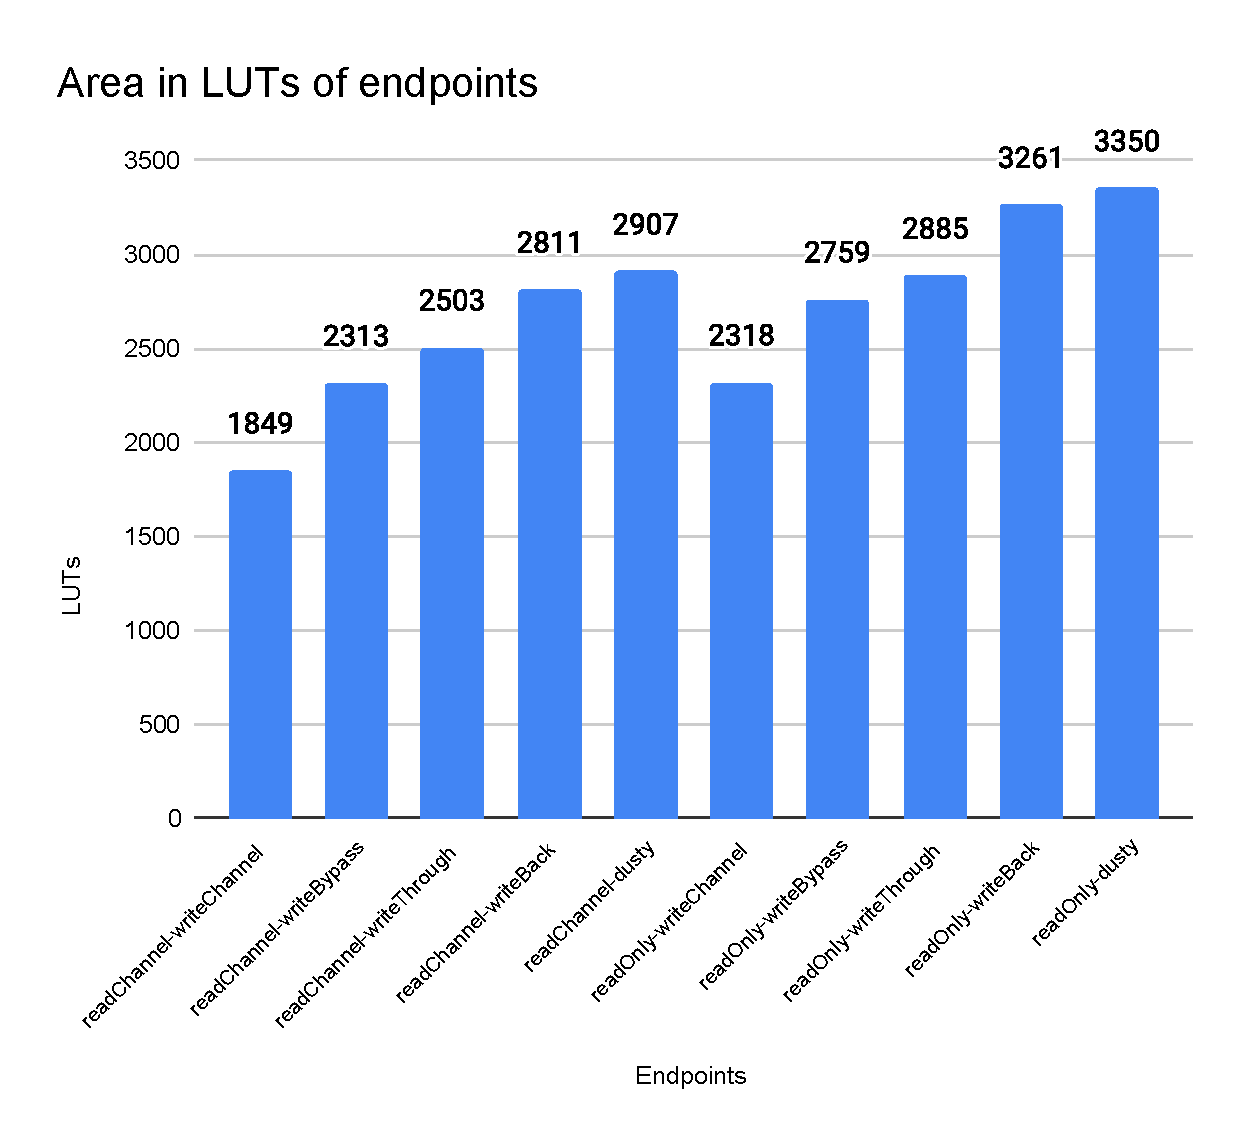
\includegraphics[width=0.5\textwidth]{isca2023-latex-template/figures/Area in LUTs of endpoints.pdf}
    \caption{Examples of before and after advice on a small toy FSM.}
    \label{fig:area}
\end{figure}

\section{Performance and Area}

We have taken our feature-oriented designs all the way up through simulation and synthesis. The hardware generator is implemented in Chisel 3.5.1. All designs were emitted as Verilog. Beyond the cache, the rest of the RISC-V Mini was kept original, implementing the RV32I ISA of the User-level Version 2.0~\cite{} and the Machine-level ISA of the Privileged Architecture Version 1.7~\cite{}. We simulated the large benchmarks from the RISC-V tests repository~\cite{RvTest} using Verilator 4.214~\cite{}. Designs were synthesized for an xc7a100tcsg324-1 FPGA using Vivado 2022.1 with the Vivado synthesis defaults. Figure \ref{fig:CPI} shows the cycles per instruction for each benchmark with the average CPI of all the benchmarks displayed at the bottom. Figure \ref{fig:area} shows the synthesized area of the whole synthesized chip design in LUTs. 

The smallest endpoint, \textbf{readChannel-writeChannel} takes only 55.2\% of the area of our largest endpoint, \textbf{readOnly-dusty}, with a reduction of CPI by 47.5\%. By feature-orienting our design, we have enabled a fine grain of design space exploration. The CPI drops nearly linearly as more features are added to the design. Coarse grained analysis is not lost in this technique either. Comparing the two instruction cache endpoint groups we see that the addition of an instruction cache has an average decrease in CPI of 1.19 cycles and an average increase in LUTs of 438. 

While this result is not surprising, adding an instruction cache should improve performance at the cost of increasing design area, we speculate that this technique can help to quickly identify the properties of new designs and save designers time. For instance, the \textbf{readOnly-writeChanel} has a lower CPI than any of the \textbf{readChannel endpoints} and takes less area than all of them except \textbf{readChannel-writeChannel}. This analysis tells us going down the path of more advanced data cache features is not worth the area cost if there is no data cache. Again, this is not surprising, but we posit that there are other opportunities in hardware designs for this sort of analysis.

A feature-oriented approach can help hardware designers better balance trade-offs while maintaining high levels of design reuse. Without the need to start hardware designs from scratch, designers can accomplish quicker prototyping while maintaining a high level of analysis and code reuse.

\section{Conclusion}

%%%%%%% -- PAPER CONTENT ENDS -- %%%%%%%%


%%%%%%%%% -- BIB STYLE AND FILE -- %%%%%%%%
\bibliographystyle{IEEEtranS}
\bibliography{refs, networks, bibdbase}
%%%%%%%%%%%%%%%%%%%%%%%%%%%%%%%%%%%%

\end{document}

